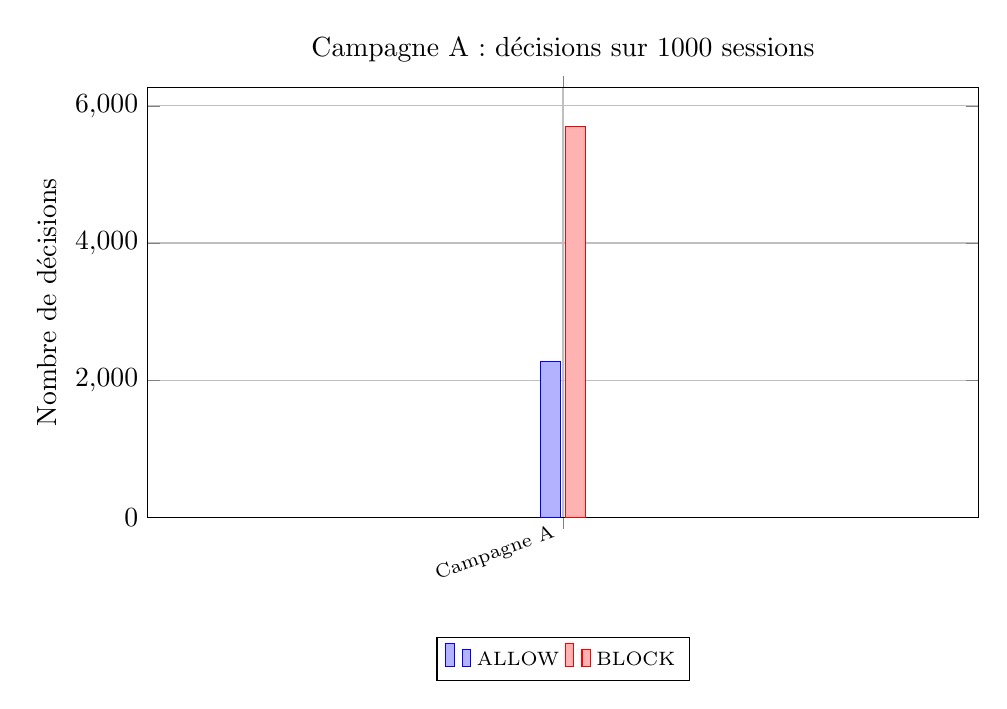
\begin{tikzpicture}
\begin{axis}[ybar,
bar width=7pt,
width=\linewidth,
height=0.58\linewidth,
title={Campagne A : décisions sur 1000 sessions},
ylabel={Nombre de décisions},
xtick={0},
xticklabels={{Campagne A}},
x tick label style={rotate=20,anchor=east,font=\scriptsize},
grid=major,
legend style={font=\scriptsize,at={(0.5,-0.28)},anchor=north,legend columns=2},
ymin=0]
\addplot+ coordinates {(0,2266)};
\addlegendentry{ALLOW}
\addplot+ coordinates {(0,5694)};
\addlegendentry{BLOCK}
\end{axis}
\end{tikzpicture}
